\chapter{Big data acquisition and processing in high-throughput label-free cell screening}
\label{chp:CLEO2015_Chapter}

Coherent-STEAM is a quantitative phase microscopy technique for label-free analysis of up to 100,000 cells per second in flow. Here, we introduce a data acquisition scheme that enables interruptionless storage of Coherent-STEAM cell images. Our proof of principle demonstration is capable of saving 10.8 TB of cell images in an hour, i.e. pictures of every single cell in 2.7 mL of a sample.

\section{Introduction}

In Coherent-STEAM system, the output signal of the photodetector usually has a very large bandwidth in the order of a few GHz. Based on Nyquist theorem, an analog-to-digital converter (ADC) with a sampling rate of at least twice the bandwidth is required to capture this signal without aliasing. If we want to capture images of every single cell in a sample, all of the ADC output samples should be recorded on a storage unit. For example, to capture and process the data for the Coherent-STEAM setup described in Chapter \ref{chp:BOE2013_Chapter}, the minimum sampling rate of the photodetector signal is 12 GS/s. If the bit-depth of the ADC is 8 bits, the acquisition system should handle storage of 12 GB of data per second. To ease the storage requirement by a few times, we purpose analog preprocessing of Coherent-STEAM data. Our technique is based on using telecommunication radio-frequency (RF) components to convert the photodetector output signal into a set of lower bandwidth signals with only the quantitative phase and intensity information, so that the sampling rate of the required ADCs can be much smaller. As a result, the storage units can handle logging these lower rate signals at real-time. Also, by parallel processing of the stored data, we would be able to retrieve the phase and intensity images in real-time and use them for cell sorting.

\section{Technical description of the acquisition system}

We have previously \cite{mahjoubfar2014label} shown that if the arms' length mismatch in Coherent-STEAM interferometer is chosen long enough, one can see two separate features in the spectrum of the system output corresponding to intensity and phase components of the cells (Figure \ref{fig:CLEO2015_Figure1}). By filtering out the high-frequency features and down-converting them to baseband, we should be able to reconstruct intensity and phase images of the cells. 

\begin{figure}[htb!]
\centering
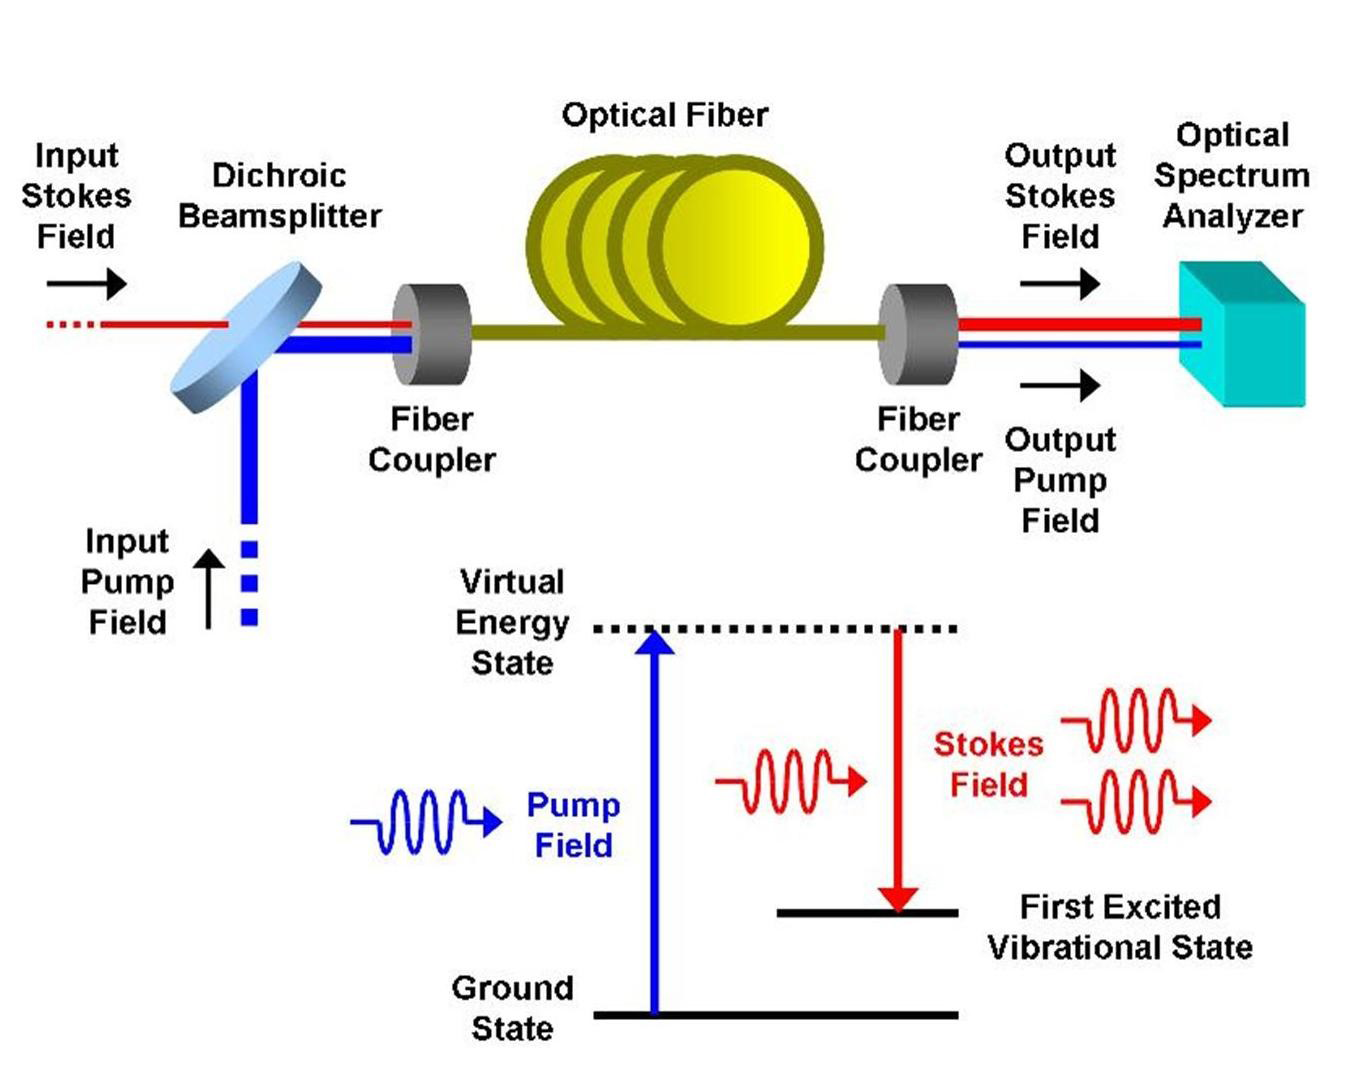
\includegraphics[scale=0.8]{CLEO2015/Figure1.png}
\caption{Spectral components of Coherent-STEAM signal. For a Coherent-STEAM setup with long enough arms' length mismatch the spectrum of the output signal shows two separate spectral bands. The low frequency components correspond to the intensity of the sample, while the high frequency components contain the phase information in addition to the intensity information of the cells.}
\label{fig:CLEO2015_Figure1}
\end{figure}

We purpose a quadrature phase demodulation scheme to perform the analog preprocessing on Coherent-STEAM signals (Figure \ref{fig:CLEO2015_Figure2}). First, the photodetector output signal is bandpass filtered and split into two paths. These signals are mixed with two sinusoidal signals that are $90^{\circ}$ phase-shifted with respect to each other. The frequency of the sinusoidal signals is approximately at the center of the high frequency features of Coherent-STEAM setup, which is set by the arms' length mismatch (in our example about 5 GHz). Mixers shift the high-frequency component containing the phase and intensity information to lower frequencies close to baseband. 

\begin{figure}[htb!]
\centering
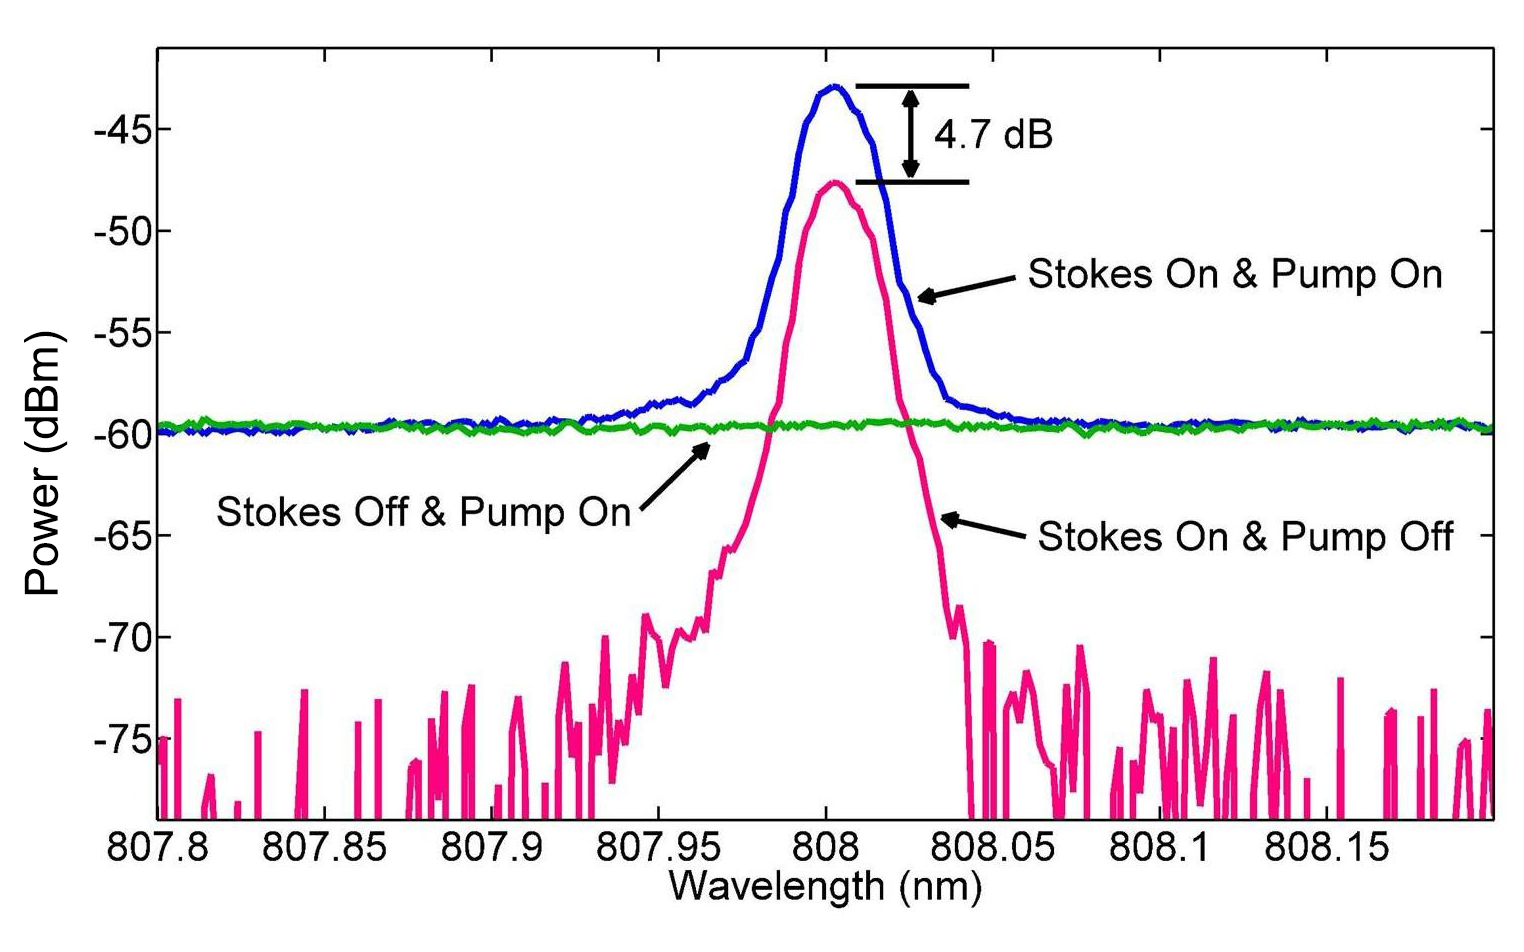
\includegraphics[scale=0.58]{CLEO2015/Figure2.png}
\caption{Analog preprocessing of Coherent-STEAM signal. The analog signal processing system for reducing the data rate of Coherent-STEAM is essentially a quadrature down-conversion unit. I and Q outputs and their corresponding spectra show that the down-conversion is effective in reducing the bandwidth and the required sampling rate.}
\label{fig:CLEO2015_Figure2}
\end{figure}

Finally, the baseband components, which now contain the sample's phase and intensity information can be filtered out and digitized with two ADCs (Figure \ref{fig:CLEO2015_Figure3}) that have a considerably smaller sampling rate than what was required before the down-conversion. In our demonstration, the sampling rate was reduced from 12 GS/s to 1.5 GS/s. In addition, since the outputs are mixed with $90^{\circ}$ phase-shifted sinusoidal signals, the phase and intensity of the signal can be respectively derived by simple calculations as
\begin{eqnarray}
\Delta\varphi = \textrm{unwrap}(\arg(\frac{I(t)}{Q(t)})), \\
\Delta I = \sqrt{I(t)^2 + Q(t)^2},
\end{eqnarray}
where $I(t)$ and $Q(t)$ are the in-phase and quadrature-phase outputs of the analog preprocessing unit as shown in Figure \ref{fig:CLEO2015_Figure2}. 

\begin{figure}[htb!]
\centering
\includegraphics[scale=0.58]{CLEO2015/Figure3.png}
\caption{Digital signal processing system for acquisition of analog preprocessing unit outputs. This system is built with simple blocks such as argument calculator, unwrapper, and first in, first outs (FIFOs), which can be performed in real-time.}
\label{fig:CLEO2015_Figure3}
\end{figure}  

\section{Big data acquisition results}

We tested the applicability of our method with a preliminary setup. To generate $90^{\circ}$ phase-shifted sinusoidal signals, we used a signal generator connected to a $90^{\circ}$ hybrid coupler. The $I(t)$ and $Q(t)$ outputs of the analog signal processing system are captured with two 1.5 GS/s analog-to-digital converters. These signals are down-converted in frequency domain and about 8 times slowed-down in time compared to the original Coherent-STEAM output (Figure \ref{fig:CLEO2015_Figure2}). This down-conversion happens for consecutive line images at real-time. Also, with careful design, both channels can have the same group delay, and edges of the pulses in two channels can align in time. 

Figure \ref{fig:CLEO2015_Figure4} shows a few intensity and phase cell images captured by our continuously recording big data acquisition system. The setup can acquire 10.8 TB of these images over a course of an hour-long experiment, which corresponds to pictures of every single cell in 2.7 mL of the suspended cells sample. The storage unit is a RAID 0 array of hard disk drives that are written and read in parallel to provide superior access speed. To capture larger data sizes, the system can be easily expanded by increasing the number of hard disk drives in the array or using larger hard drives. 

\begin{figure}[htb!]
\centering
\includegraphics[scale=0.6]{CLEO2015/Figure4.png}
\caption{Sample images acquired by the analog preprocessing system. Both phase and intensity images for two different sets of OT-II hybridoma T cells in flow are shown.}
\label{fig:CLEO2015_Figure4}
\end{figure}  

Also, the required digital signal processing for derivation of sample phase-shift from the outputs of the analog signal processing system, $I(t)$ and $Q(t)$, can be easily implement on an FPGA. Figure \ref{fig:CLEO2015_Figure3} shows a suggested design for such an FPGA unit. One can see that it only requires implementation of basic blocks such as argument calculator, unwrapper, and first in, first outs (FIFOs). This is a direct result of transferring the cumbersome and calculation intensive operations of the phase recovery algorithm (such as Hilbert transformation) to the analog preprocessing unit. This way, the FPGA output signal can be directly used to control a cell sorter in our label-free imaging flow cytometer. 

\section{Conclusion}

In summary, we used quadrature phase demodulation technique to reduce the sampling rate required for capturing Coherent-STEAM signals, decrease the amount of data that is generated, and facilitate the data processing. As a proof of principle, we showed an acquisition system capable of continuously recording 10.8 TB of phase and intensity images. 